\xiti
\begin{xiaotis}

\xiaoti{画两个相交平面,在一个平面内画一条直线和另一平面平行。}

\xiaoti{}%
\begin{xiaoxiaotis}%
    \xxt[\xxtsep]{一条直线和另一条直线平行,它就和经过另一条直线的任何平面平行。这是否正确?}

    \xxt{一条直线和一个平面平行,它就和这个平面内的任何直线平行。这是否正确?}

    \xxt{平行于同一平面的两条直线互相平行。这是否正确?}

\end{xiaoxiaotis}


\xiaoti{求证:如果一条直线与两个相交的平面都平行,那么这条直线与这两个平面的交线平行。}

\xiaoti{求证:经过两条异面直线中的一条,有一个平面与另一条直线平行。}

\xiaoti{求证:如果一条直线与一个平面平行,那么夹在这条直线和平面间的平行线段相等。}

\xiaoti{求证:如果两条平行线中的一条和一个平面相交,那么另一条也和这个平面相交。}

\xiaoti{如果一条直线与一个平面平行,那么过这个平面内的一点与这条直线平行的直线,必在这个平面内。}

\xiaoti{直线 $AB$ 平行于平面 $\alpha$, 经过 $AB$ 的一组平面和平面 $\alpha$ 相交。
    求证:它们的交线 $a$、$b$、$c$、…是一组平行线。
}

\begin{figure}[htbp]
    \centering
    \begin{minipage}[b]{7cm}
        \centering
        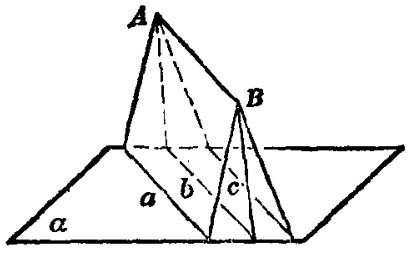
\includegraphics[width=6cm]{../pic/ltjh-ch1-xiti3-08.png}
        \caption*{(第 8 题)}
    \end{minipage}
    \qquad
    \begin{minipage}[b]{4cm}
        \centering
        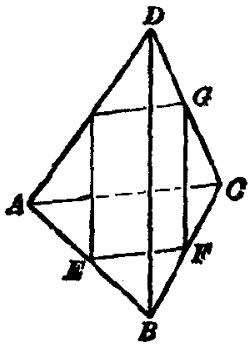
\includegraphics[width=4cm]{../pic/ltjh-ch1-xiti3-09.png}
        \caption*{(第 9 题)}
    \end{minipage}
\end{figure}


\xiaoti{已知:空间四边形 $ABCD$,$E$、$F$、$G$ 分别是 $AB$、$BC$、$CD$ 的中点。
    求证:平面 $EFG \pingxing BD$,平面 $EFG \pingxing AC$。
}

\xiaoti{求证:如果两个相交平面分别经过两条平行直线中的一条,那么它们的交线和这两条直线平行。}

\end{xiaotis}

